\section{Results}

The results include the time-dependent resources required 
for each of the transition scenarios described. This includes 
the number of reactors, mass of enriched uranium, and the 
\gls{SWU} capacity needed to produce the enriched uranium.
Results presented here include the simulations of the 
current U.S. fuel cycle and no growth transition scenarios. 

Figure \ref{fig:rx_deployment} shows the total number 
of each type of reactors deployed in each of the simulated 
scenarios. All scenarios deploy the same number of \gls{LWR}s. 
Each of the transitions utilize a \Cycamore ``GrowthRegion'' 
to control the deployment of the advanced reactor as needed 
to meet the specified demand. All of the scenarios deploy the 
\gls{LWR}s at the same time. For each of the transitions 


\begin{figure}[ht]
    \centering
    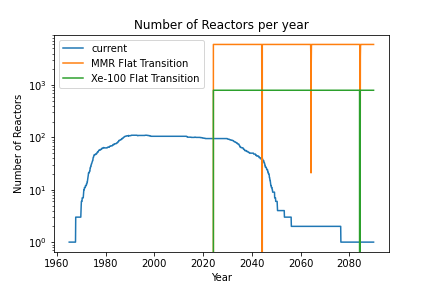
\includegraphics[scale=0.5]{figures/rx_deployment_all.png}
    \caption{Deployment  in each scenario.}
    \label{fig:rx_deployment}
\end{figure}

Figure \ref{fig:energy} shows the total energy output from 
all of the reactors in each scenario. Each of the scenarios
have very similar energy outputs, until  when the transitions 
begin to have most of their energy from the advanced reactors.
The energy output in 
each of the transition scenarios does not match the flat demand 
starting at 2025 specified by the \Cycamore ``GrowthRegion''. 
This is due to 
the use of mutual transactions in the dynamic resource exchange
(DRE) \cite{gidden_methodology_2016}, which requires that each 
material request filled must be filled in full. A cap had to be 
placed on the inventory of feed material (UF$_6$ commodity) that 
the enrichment facility could store. Further work is required 
to determine the cap on feed material inventory to better meet 
the intended energy demand of the transitions. The transition to 
the Xe-100 reactor better matches the energy demand than the 
transition to the \gls{MMR} reactor, most likely because of the 
longer lifetime of the Xe-100 reactor. 

\begin{figure}[ht]
    \centering
    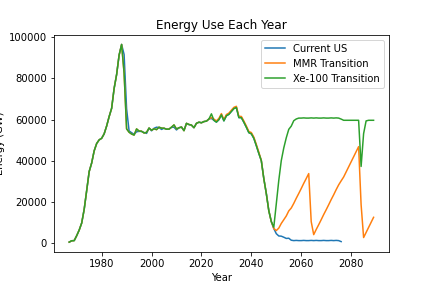
\includegraphics[scale=0.5]{figures/energy_all.png}
    \caption{Energy output of all reactors in each scenario.}
    \label{fig:energy}
\end{figure}

Figure \ref{fig:enriched_u} shows the amount of \gls{HALEU} 
required by the advanced reactors in the transition scenarios. 
Both scenarios show a spike in \gls{HALEU} demand in 1975, which 
an artifact of the DRE, and not due to the reactors requiring the 
fuel. Looking at the demand of \gls{HALEU} after 2049, the 
\gls{MMR} transition requires 4556-6409 kg more than the 
Xe-100 transition, except for a single time step in 2084 when 
the Xe-100 transition requires almost 69,000 kg more. 

\begin{figure}[ht]
    \centering
    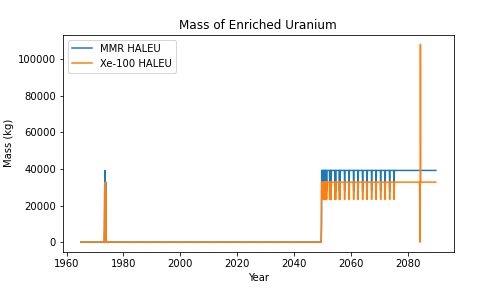
\includegraphics[scale=0.5]{figures/enrichedU_advancedrx.png}
    \caption{Enriched uranium demand for reactors.}
    \label{fig:enriched_u}
\end{figure}

Finally, Figure \ref{fig:swu} shows the \gls{SWU} required to 
produce enriched uranium in each scenario. The calculated 
\gls{SWU} for the transition scenarios includes \gls{SWU} to 
produce \gls{HALEU} for the advanced reactor and the \gls{LEU}
to produce fuel for the \gls{LWR}s. There is a clear increase 
in \gls{SWU} from the current fuel cycle simulation to the 
transition scenarios once the advanced reactors are fueled. 
For most of the time steps in which the advanced reactors 
require fuel, the Xe-100 transition requires 22,881 kg-SWU 
more than the MMR transition scenario, despite the MMR 
transition requiring a larger mass of \gls{HALEU}. This is 
because the Xe-100 reactors require a higher level of 
enrichment.  

\begin{figure}[ht]
    \centering
    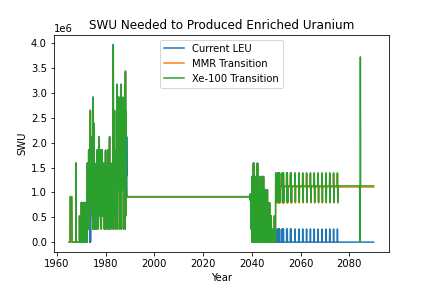
\includegraphics[scale=0.5]{figures/swu_all.png}
    \caption{Enriched uranium demand for reactors.}
    \label{fig:swu}
\end{figure}